\documentclass[../main.tex]{subfiles}

\begin{document}

\section{Manual de instalación}

Para que se pueda ejecutar el código y visualizar los resultados se requiere la distribución Anaconda.
Además, es necesario instalar las librerías de Python: PyPdf2, pdfminer.six, langdetect y wordcloud.

El sistema operativo que se ha empleado es la distribución de Linux OpenSUSE Tumbleweed. Los pasos que se muestran en este manual están basados en dicha distribución.

\textbf{\large{Requisitos:}}

\begin{itemize}
	\item Licencia: uso y distribución libre bajo los términos del Acuerdo de Licencia de Usuario Final de Anaconda Distribution.
	\item Sistema operativo: Windows 8 o posterior, macOS 10.13+, o Linux.
	\item Arquitectura de sistema: 64-bit x86 y 32-bit x86 (solo Windows)
	\item Espacio en disco: mínimo 5 GB para la descarga e instalación.
\end{itemize}

\textbf{\large{Instalación en Linux:}}

\textbf{Prerrequisitos}

Para utilizar los paquetes de la interfaz gráfica con Linux, se deben instalar las siguientes dependencias con Qt:

\begin{itemize}
	\renewcommand\labelitemi{--}
	\setlength\itemsep{-1em}
	\item libXcomposite1
	\item libXi6
	\item libXext6
	\item libXau6
	\item libX11-6
	\item libXrandr2
	\item libXrender1
	\item libXss1
	\item libXtst6
	\item libXdamage1
	\item libXcursor1
	\item libxcb1
	\item libasound2
	\item libX11-xcb1
	\item Mesa-libGL1
	\item Mesa-libEGL1
\end{itemize}

Se puede comprobar si se encuentran instalados con el comando:

\begin{lstlisting}[language=bash]
	zypper search libXcomposite1 libXi6 libXext6 libXau6 libX11-6 libXrandr2 libXrender1 libXss1 libXtst6 libXdamage1 libXcursor1 libxcb1 libasound2  libX11-xcb1 Mesa-libGL1 Mesa-libEGL1
\end{lstlisting}

Si no se encontraran en el sistema, se instalan con el siguiente comando:

\begin{lstlisting}[language=bash]
	zypper install libXcomposite1 libXi6 libXext6 libXau6 libX11-6 libXrandr2 libXrender1 libXss1 libXtst6 libXdamage1 libXcursor1 libxcb1 libasound2  libX11-xcb1 Mesa-libGL1 Mesa-libEGL1
\end{lstlisting}

\textbf{Descarga}

Desde el navegador, acceder a la web de Anaconda y seleccionar el instalador de Linux.

\begin{figure}[h]
	\centering
	
\includegraphics[width=0.7\linewidth]{../images/anaconda-install-01}
	\caption{Página de inicio de la web de Anaconda \cite{anaconda2022web}}
	\label{fig:anaconda-install-01}
\end{figure}

Una vez descargado el fichero, se recomienda verificar la integridad del mismo. Desde el terminal se ejecuta el siguiente comando:

\begin{lstlisting}[language=bash]
	shasum -a 256 Anaconda3-2022.05-Linux-x86_64.sh
\end{lstlisting}

El resultado debe coincidir con el \textit{hash} facilitado por Anaconda en su web \url{https://docs.anaconda.com/anaconda/install/hashes/}.

\textbf{Instalación}

Desde la terminal hay que situarse en la carpeta de descargas. Luego hay que lanzar el ejecutable con Bash:

\begin{lstlisting}[language=bash]
	bash ./Anaconda3-2020.05-Linux-x86_64.sh
\end{lstlisting}

Se solicita la revisión del acuerdo de licencia. Hay que pulsar \texttt{Enter} para continuar. Una vez leído, se introduce «yes» si se aceptan los términos y se quiere continuar con la instalación.

A continuación se solicita la ruta de instalación. Se recomienda utilizar la ruta por defecto (Figura \ref{fig:anaconda-install-02}).

\begin{figure}[h]
	\centering
	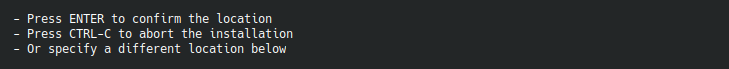
\includegraphics[width=0.7\linewidth]{../images/anaconda-install-02}
	\caption{Mensaje de instalación de Anaconda}
	\label{fig:anaconda-install-02}
\end{figure}

Una vez finalazada la instalación, hay que elegir si se inicializa Anaconda Distribution. Se recomienda aceptar la ejecución de \texttt{conda init}. Si no se aceptara, no se modificará el \textit{shell} y habrá que activar conda cada vez que se quiera lanzar.

\textbf{Verificación}

Tras la instalación, se puede verificar que todos los paquetes están instalados en el sistema ejecutando desde la terminal el comando:

\begin{lstlisting}[language=bash]
	conda list
\end{lstlisting}

Por pantalla deben aparecer todos los paquetes de conda junto con su versión, como se muestra en la Figura \ref{fig:anaconda-install-03}.

\begin{figure}[h]
	\centering
	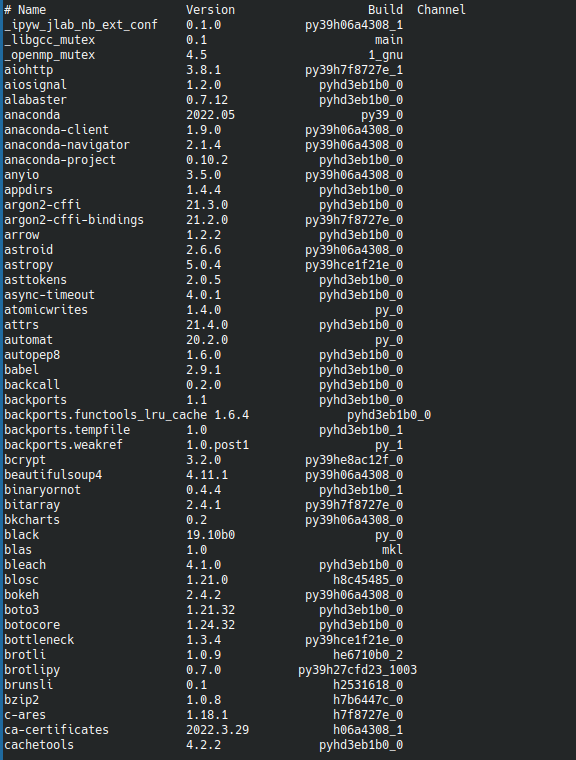
\includegraphics[width=0.7\linewidth]{../images/anaconda-install-03}
	\caption{Listado de paquetes instalados}
	\label{fig:anaconda-install-03}
\end{figure}

Por último, también desde la terminal, se ejecuta el comando:

\begin{lstlisting}[language=bash]
	anaconda-navigator
\end{lstlisting}

Este abrirá la ventana de Anaconda Navigator. Esta aplicación sirve de lanzador de todo el software que incluye Anaconda (Figura \ref{fig:anaconda-navigator}).

\begin{figure}[h]
	\centering
	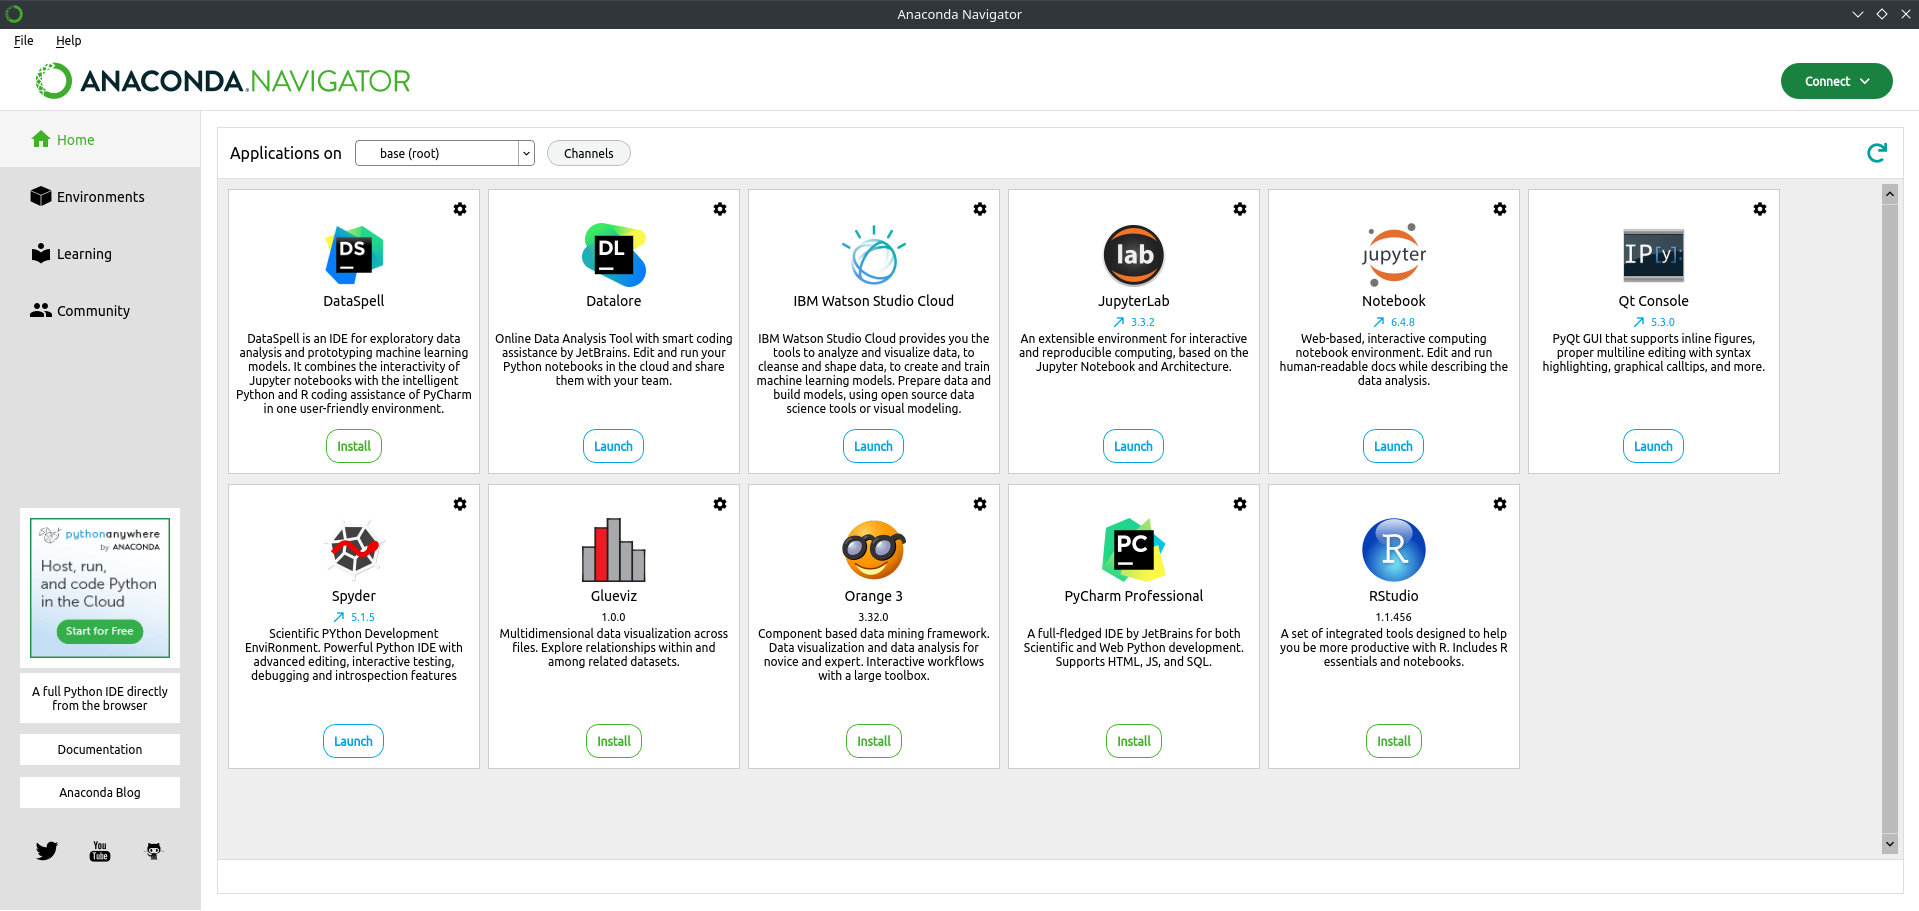
\includegraphics[width=0.7\linewidth]{../images/anaconda-navigator}
	\caption{Captura de la pantalla de inicio de Anaconda Navigator}
	\label{fig:anaconda-navigator}
\end{figure}

\textbf{Librería adicionales}

Además de todos los paquetes que incluye conda, es necesario instalar cuatro librerías adicionales. Estas son utilizadas para la lectura de los PDF, la detección del idioma y la generación de nubes de palabras.

La instalación se realiza desde la terminal. Hay dos métodos para hacerlo:

\begin{itemize}
	\item El repositorio Python Package Index (PyPI). Se utiliza el comando \texttt{pip}.
	\item La colección de software conda-forge mantenido por la comunidad. Se utiliza el comando \texttt{conda}.
\end{itemize}

Instalación mediante PyPI:

\begin{lstlisting}[language=bash]
	pip install langdetect
	pip install pdfminer.six
	pip install PyPDF2
	pip install wordcloud
\end{lstlisting}

Instalación mediante conda-forge:

\begin{lstlisting}[language=bash]
	conda install -c conda-forge langdetect
	conda install -c conda-forge pdfminer.six
	conda install -c conda-forge pypdf2
	conda install -c conda-forge wordcloud
\end{lstlisting}


\end{document}
